% ---------------------------------------------------------------
% TEMPLATE TCC1 - SENAC SANTO AMARO
% ---------------------------------------------------------------
% Trabalho de Conclusão de Curso 1
% Elaborado para apresentação da proposta inicial do TCC
% Estrutura: 4 capítulos (Introdução, Revisão Bibliográfica,
%            Desenvolvimento, Referências Bibliográficas)
% ---------------------------------------------------------------

\documentclass[
    12pt,                % tamanho da fonte
    openright,           % capítulos começam em página ímpar
    oneside,             % para impressão em apenas um lado do papel
    a4paper,             % tamanho do papel
    english,             % idioma adicional
    brazil               % idioma principal
]{abntex2}

% ---------------------------------------------------------------
% PACOTES
% ---------------------------------------------------------------
\usepackage{lmodern}                % Fonte Latin Modern
\usepackage[T1]{fontenc}            % Seleção de códigos de fonte
\usepackage[utf8]{inputenc}         % Codificação do documento
\usepackage{lastpage}               % Usado pela Ficha catalográfica
\usepackage{indentfirst}            % Indenta o primeiro parágrafo
\usepackage{color}                  % Controle de cores
\usepackage{graphicx}               % Inclusão de gráficos
\usepackage{microtype}              % Melhorias de justificação
\usepackage{float}                  % Para posicionamento de figuras
\usepackage{booktabs}               % Tabelas profissionais
\usepackage{multirow}               % Células mescladas em tabelas
\usepackage{longtable}              % Tabelas longas
\usepackage{amsmath,amssymb}        % Símbolos matemáticos
\usepackage{pgfgantt}               % Diagramas de Gantt
\usepackage[brazilian,hyperpageref]{backref}  % Páginas com citações
\usepackage[alf]{abntex2cite}       % Citações ABNT

% ---------------------------------------------------------------
% CONFIGURAÇÕES DO PDF
% ---------------------------------------------------------------
\makeatletter
\hypersetup{
    pdftitle={\@title},
    pdfauthor={\@author},
    pdfsubject={TCC1 - SENAC Santo Amaro},
    pdfcreator={LaTeX with abnTeX2},
    pdfkeywords={tcc}{senac}{santo amaro}{trabalho de conclusão},
    colorlinks=true,        % false: links em caixas; true: links coloridos
    linkcolor=blue,         % cor dos links internos
    citecolor=blue,         % cor dos links para bibliografia
    filecolor=magenta,      % cor dos links para arquivos
    urlcolor=blue,
    bookmarksdepth=4
}
\makeatother

% ---------------------------------------------------------------
% CONFIGURAÇÕES DE APARÊNCIA DO PDF FINAL
% ---------------------------------------------------------------
\definecolor{blue}{RGB}{41,5,195}

% ---------------------------------------------------------------
% INFORMAÇÕES DO DOCUMENTO
% ---------------------------------------------------------------
\titulo{Otimização de Rotas Internas no Senac Considerando a Qualidade do Wi-Fi: Uma Comparação 
entre Algoritmo de Grafos e Inteligência Artificial} %Trocar titulo
\autor{
Edinaldo Matias dos Santos Junior \\
André Luis Ferreira de Oliveira}
\local{São Paulo}
\data{2026}
\orientador{Prof. Thyago Quintas}
% \coorientador{Prof. Nome do Coorientador} % Descomente se houver coorientador

\instituicao{%
  SENAC -- Serviço Nacional de Aprendizagem Comercial
  \par
  Unidade Santo Amaro
  \par
  Curso de Ciência da Computação
}

\tipotrabalho{Trabalho de Conclusão de Curso I}

\preambulo{Proposta de Trabalho de Conclusão de Curso apresentado ao SENAC Santo Amaro como requisito parcial para aprovação na disciplina de TCC1 do curso de Ciência da Computação.}

% ---------------------------------------------------------------
% COMPILA O ÍNDICE
% ---------------------------------------------------------------
\makeindex

% ---------------------------------------------------------------
% INÍCIO DO DOCUMENTO
% ---------------------------------------------------------------
\begin{document}

% Seleciona o idioma do documento
\selectlanguage{brazil}

% Retira espaço extra obsoleto entre as frases
\frenchspacing

% ---------------------------------------------------------------
% ELEMENTOS PRÉ-TEXTUAIS
% ---------------------------------------------------------------
\pretextual

% ---------------------------------------------------------------
% CAPA
% ---------------------------------------------------------------
\imprimircapa

% ---------------------------------------------------------------
% FOLHA DE ROSTO
% ---------------------------------------------------------------
\imprimirfolhaderosto

% ---------------------------------------------------------------
% RESUMO
% ---------------------------------------------------------------
% ---------------------------------------------------------------
% RESUMO
% ---------------------------------------------------------------
\begin{resumo}
Este documento apresenta a proposta inicial do Trabalho de Conclusão de Curso (TCC1) desenvolvido no Centro Universitário SENAC Santo Amaro. O objetivo deste trabalho é comparar a eficácia do algoritmo determinístico de Dijkstra com um modelo de Inteligência Artificial baseado em Aprendizado por Reforço (\textit{Q-Learning}) na otimização de rotas internas, utilizando a estabilidade do sinal Wi-Fi (RSSI) como variável de custo dinâmico. A justificativa para este estudo baseia-se na ineficácia do GPS em espaços fechados e na vulnerabilidade de abordagens clássicas de roteamento estático frente às flutuações estocásticas de sinais sem fio em Ambientes Dinâmicos (DE). A revisão bibliográfica abrange as limitações dos sistemas de posicionamento \textit{indoor} (IPS), a teoria dos grafos aplicada à descoberta de caminhos, a métrica RSSI e os fundamentos do roteamento adaptativo (\textit{Q-Routing}). Como solução proposta, pretende-se inicialmente modelar os corredores do Prédio Acadêmico I da instituição como uma rede de grafos, compilar um banco de dados empírico das variações do sinal Wi-Fi através da plataforma \textit{IndoorAtlas} e submeter ambos os algoritmos a testes comparativos sob duas condições: cenários de controle (representando estabilidade de conexão) e cenários de estresse (simulando quedas abruptas de sinal e congestionamento de rede), provando a capacidade da IA em priorizar a conectividade em detrimento da distância física. Este trabalho está organizado em capítulos que apresentam a introdução ao tema, a revisão bibliográfica que fundamenta a pesquisa, o desenvolvimento com a solução proposta e o cronograma de trabalho, seguidos das referências bibliográficas.

\vspace{\onelineskip}

\noindent
\textbf{Palavras-chave}: Navegação \textit{Indoor}. Teoria dos Grafos. Dijkstra. \textit{Q-Learning}. RSSI.
\end{resumo}

% ---------------------------------------------------------------
% LISTA DE ILUSTRAÇÕES
% ---------------------------------------------------------------
% \pdfbookmark[0]{\listfigurename}{lof}
% \listoffigures*
% \cleardoublepage

% ---------------------------------------------------------------
% LISTA DE TABELAS
% ---------------------------------------------------------------
% \pdfbookmark[0]{\listtablename}{lot}
% \listoftables*
% \cleardoublepage

% ---------------------------------------------------------------
% SUMÁRIO
% ---------------------------------------------------------------
\pdfbookmark[0]{\contentsname}{toc}
\tableofcontents*
\cleardoublepage

% ---------------------------------------------------------------
% ELEMENTOS TEXTUAIS
% ---------------------------------------------------------------
\textual

% ===============================================================
% CAPÍTULO 1 - INTRODUÇÃO
% ===============================================================
\chapter{Introdução}
\label{cap:introducao}

O sistema de posicionamento e navegação em ambientes externos (\textit{outdoor}) consolidou-se como uma tecnologia altamente eficiente, fornecendo a localização precisa de objetos e usuários por meio de sinais de satélite, como o Sistema de Posicionamento Global (GPS). No entanto, esse método opera de forma eficaz apenas em áreas abertas com linha de visão direta. Quando o usuário adentra edifícios, os sinais sofrem interferência severa ou bloqueio completo por paredes e telhados, tornando o GPS ineficaz para navegação interna \cite{Chia2025,BarrosoBrito2025}. 

Para solucionar a navegação nesses espaços fechados, \citeonline{Stancel2021} afirmam que o mundo real pode ser mapeado computacionalmente através de um grafo de vértices e arestas. A viabilidade dessa modelagem estrutural especificamente para os corredores do Senac já foi comprovada empiricamente por \citeonline{BarrosoBrito2025}. A partir dessa modelagem, algoritmos clássicos de teoria dos grafos, como Dijkstra e A*, são muito bem-sucedidos ao definir a menor rota para redes com custos de arestas estáticos. Entretanto, no contexto prático real, os custos das arestas mudam dinamicamente.

Sendo assim, essas abordagens tradicionais apresentam várias limitações em cenários onde o usuário terá sua rota determinada a fim de evitar congestionamentos ou manter uma conectividade Wi-Fi \cite{Pham2025}.

Para \citeonline{Pham2025}, algoritmos baseados em aprendizado por reforço computam ótimos resultados quando tratamos de redes que mudam dinamicamente. Dessa forma, este estudo propõe realizar um comparativo prático no Centro Universitário Senac entre o algoritmo determinístico de Dijkstra e um modelo de Inteligência Artificial (IA) baseado em Aprendizado por Reforço (RL), utilizando como pesos das arestas a distância física (metros) e a qualidade do sinal baseada no Received Signal Strength Indicator (RSSI).

% ---------------------------------------------------------------

\section{Contexto}
\label{sec:contexto}

O desenvolvimento de sistemas de posicionamento e navegação revolucionou a mobilidade e a interação espacial na sociedade contemporânea. Em ambientes externos (\textit{outdoor}), tecnologias baseadas em constelações de satélites, como o Sistema de Posicionamento Global (GPS), consolidaram-se como soluções altamente eficientes para o rastreamento preciso de usuários. No entanto, a eficácia desse método restringe-se a áreas abertas com linha de visão direta. Quando o indivíduo adentra edifícios e complexos arquitetônicos fechados, os sinais de rádio sofrem interferência severa ou bloqueio total por estruturas físicas, como paredes e lajes, tornando o GPS ineficaz para a navegação interna (\textit{indoor}) \cite{Chia2025, BarrosoBrito2025}.

Para viabilizar o deslocamento nesses espaços fechados, a literatura e a indústria têm recorrido a infraestruturas locais preexistentes, com destaque para a utilização de redes sem fio (Wi-Fi). Computacionalmente, o ambiente físico de uma instituição pode ser mapeado e abstraído por meio de uma estrutura de grafos, composta por vértices e arestas que representam os cruzamentos e os corredores \cite{Stancel2021}. Para quantificar o peso ou custo dessas arestas visando a manutenção da conectividade, a métrica de Indicador de Força do Sinal Recebido (RSSI), expressa em decibéis por miliwatt (dBm), estabeleceu-se como um padrão de medição. 

Entretanto, o domínio físico em que esse sistema opera caracteriza-se por ser um Ambiente Dinâmico (DE - \textit{Dynamic Environment}). Em instituições de grande porte, o fluxo estocástico de pessoas, a movimentação de mobiliário, o ruído eletromagnético e a interferência de múltiplos caminhos (\textit{multipath interference}) causam flutuações constantes na propagação do sinal. Consequentemente, a força do sinal Wi-Fi torna-se altamente vulnerável à atenuação, resultando em uma métrica de custo dinâmico e instável \cite{Chia2025}.

A existência desse fenômeno dinâmico expõe uma lacuna crítica nas abordagens computacionais de roteamento. Algoritmos clássicos da teoria dos grafos, como o método de Dijkstra, são amplamente utilizados e comprovadamente ótimos para definir a menor rota em redes onde os custos das arestas são estáticos. Contudo, em um cenário prático e real, as abordagens determinísticas tradicionais apresentam limitações severas, pois são incapazes de adaptar o roteamento de forma reativa a custos de ligação que mudam em tempo real \cite{Pham2025}.

A incapacidade de resolver essa assimetria entre algoritmos estáticos e ambientes dinâmicos afeta diretamente os usuários finais que dependem de navegação assistida e conectividade ininterrupta em amplas instalações. A principal consequência de ignorar essas flutuações é a geração de rotas que, apesar de geograficamente mais curtas, direcionam o indivíduo para "zonas de sombra" ou áreas de alta atenuação de rede.

Diante desse cenário, o estudo de métodos adaptativos evidencia sua relevância. Para a sociedade, garante uma experiência de navegação contínua e conectada. Para a Ciência da Computação, preenche a lacuna metodológica identificada na literatura atual, investigando como técnicas emergentes de Inteligência Artificial --- especificamente o Aprendizado por Reforço, capaz de lidar com a dinamicidade de redes de forma autônoma --- podem superar os limites dos algoritmos estáticos no roteamento em ambientes complexos \cite{Pham2025}.

% ---------------------------------------------------------------
\section{Justificativa}
\label{sec:justificativa}

A motivação para o desenvolvimento deste trabalho fundamenta-se na necessidade de adequar os sistemas de roteamento \textit{indoor} à realidade estocástica das infraestruturas de rede modernas. Historicamente, o problema de caminhos mínimos tem sido tratado sob uma ótica estática, o que se mostra insuficiente frente às flutuações inerentes a ambientes com alta circulação. Diante disso, a pertinência desta pesquisa sustenta-se sob três pilares fundamentais: a identificação de uma lacuna na literatura, a sua relevância acadêmica e a sua aplicabilidade prática.
\begin{itemize}
    \item \textbf{Relevância acadêmica}: Este trabalho contribui diretamente para o avanço do conhecimento na intersecção entre a Teoria dos Grafos e a Inteligência Artificial. Ao propor um comparativo empírico entre um algoritmo determinístico clássico (Dijkstra) e um modelo adaptativo (\textit{Q-Learning}) sob a aplicação de princípios de engenharia de caos --- prática metodológica que consiste na injeção intencional de anomalias e falhas controladas (como a degradação abrupta do sinal Wi-Fi) para testar a resiliência do sistema ---, a pesquisa não se limita a revisar conceitos existentes. Ela fornece dados práticos sobre o comportamento, a convergência e a resiliência de modelos de RL na mitigação de flutuações do sinal RSSI. Essa abordagem eleva a discussão acadêmica ao demonstrar como a variabilidade do ambiente pode ser tratada matematicamente não como um ruído impeditivo, mas como uma variável de custo penalizadora na função de recompensa de um agente inteligente.
    
    \item \textbf{Relevância prática/profissional}: No âmbito aplicado, os benefícios gerados por esta solução impactam diretamente a experiência dos usuários e a gestão de infraestrutura de instituições de grande porte. O desenvolvimento de um sistema de roteamento inteligente permitirá que transeuntes --- sejam alunos, funcionários ou visitantes do Centro Universitário Senac --- desloquem-se pelas dependências do campus de maneira otimizada. A solução proposta garante não apenas a indicação do caminho fisicamente viável, mas, primordialmente, a manutenção da conectividade com a internet durante todo o trajeto. Evitar a transição por "zonas de sombra" previne a interrupção de aplicações em tempo real, chamadas de vídeo e transmissões de dados, agregando um valor operacional direto para a comunidade e servindo como um modelo escalável para hospitais, aeroportos e polos corporativos.

    \item \textbf{Lacuna identificada}: A revisão da literatura atual revela uma escassez significativa de estudos que abordem o roteamento físico sob a perspectiva dos Ambientes Dinâmicos (DE). Conforme apontado por \citeonline{Chia2025}, a grande maioria das pesquisas sobre posicionamento \textit{indoor} baseado em Wi-Fi ignora as flutuações contínuas do ambiente, assumindo premissas de estabilidade que não se verificam no mundo real. Paralelamente, embora os métodos de Aprendizado por Reforço (RL) sejam amplamente consolidados para o cálculo de rotas dinâmicas em redes lógicas de computadores, o seu potencial para redes de transporte físico e navegação humana começou a atrair atenção apenas recentemente \cite{Pham2025}. Desse modo, carece-se de estudos empíricos que unam essas técnicas de Inteligência Artificial à otimização de caminhos guiados por fatores dinâmicos de infraestrutura.
\end{itemize}
% ---------------------------------------------------------------
\section{Objetivo}
\label{sec:objetivo}

Esta seção define as metas estabelecidas para a resolução do problema de roteamento \textit{indoor} em ambientes dinâmicos, apresentando o propósito central da pesquisa e as etapas metodológicas necessárias para sua execução.

\subsection{Objetivo principal}

Comparar a eficácia do algoritmo determinístico de Dijkstra com um modelo de Inteligência Artificial baseado em Aprendizado por Reforço (\textit{Q-Learning}) na otimização de rotas internas no Centro Universitário Senac, utilizando a qualidade e a estabilidade do sinal Wi-Fi (RSSI) como variável de custo dinâmico.

\subsection{Objetivos secundários}

Os objetivos secundários representam os desdobramentos metodológicos e práticos necessários para o alcance da meta principal:

\begin{enumerate}
    \item Realizar o mapeamento topológico da planta baixa do Centro Universitário Senac, convertendo os corredores e cruzamentos da instituição em uma rede de grafos navegável;
    \item Coletar e compilar um banco de dados empírico contendo as aferições reais da potência do sinal Wi-Fi (RSSI) no ambiente estudado, mapeando as flutuações em diferentes períodos de fluxo e ocupação;
    \item Implementar o algoritmo clássico de Dijkstra para o roteamento na rede, adotando a métrica de distância física combinada com a média estática do RSSI como peso fixo das arestas;
    \item Implementar o algoritmo de \textit{Q-Learning}, realizando a modelagem matemática do ambiente (estados, ações e função de custo/recompensa) para que o agente autônomo aprenda interativamente a contornar rotas de baixa conectividade;
    \item Avaliar e comparar o desempenho de ambas as abordagens computacionais em cenários estáticos (ordem) e dinâmicos (caos), com base nos critérios de completude, grau de otimização, complexidade de tempo e complexidade de espaço.
\end{enumerate}
% CAPÍTULO 2 - REVISÃO BIBLIOGRÁFICA
% ===============================================================
\chapter{Revisão Bibliográfica}
\label{cap:revisao}

Este capítulo apresenta a fundamentação teórica que sustenta o desenvolvimento desta pesquisa. A revisão está organizada em conceitos estruturais que abordam os desafios da navegação \textit{indoor}, o comportamento estocástico da métrica RSSI, os fundamentos da Teoria dos Grafos e os preceitos da Inteligência Artificial aplicados ao roteamento dinâmico.

% ---------------------------------------------------------------
\section{Referencial teórico}
\label{sec:referencial}
\subsection{Navegação \textit{Indoor}, Wi-Fi e a Métrica RSSI}
A complexidade de localizar e guiar usuários em ambientes fechados difere drasticamente da navegação \textit{outdoor}. Enquanto espaços abertos dependem do Sistema de Posicionamento Global (GPS), a infraestrutura \textit{indoor} exige tecnologias locais devido à severa atenuação que os sinais de satélite sofrem ao atravessar barreiras arquitetônicas. Para contornar esse desafio tecnológico, \citeonline{Stancel2021} afirmam que o sinal Wi-Fi desponta como a tecnologia viável mais proeminente, permitindo o posicionamento em aeroportos, garagens e campus universitários sem a necessidade de infraestrutura de hardware adicional no dispositivo do usuário.

A principal métrica extraída dessa rede é o \textit{Received Signal Strength Indicator} (RSSI), que quantifica a força do sinal recebido por um dispositivo móvel. O valor do RSSI é expresso em decibéis por miliwatt (dBm) e é comumente lido em espectros negativos, onde valores mais próximos de zero indicam maior qualidade de conexão. 

\begin{figure}[H]
    \centering
    \caption{Figura 1 - Expressão dos decibéis por miliwatt}
    
    % 2. A imagem em si
    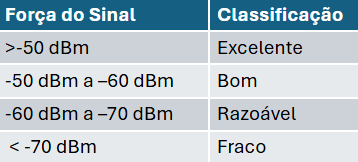
\includegraphics[width=0.5\textwidth]{img/RSSI.png}    
    % 3. A fonte fica embaixo da imagem (use \fonte)
    \fonte{Elaborado pelo autor, com base em \citeonline{Chia2025}}
    
    % 4. O apelido para você referenciar no texto
    \label{fig:dinamica_rssi}
\end{figure}

Contudo, a literatura aponta que a estabilidade dessa métrica é altamente vulnerável. Segundo \citeonline{Chia2025}, espaços internos fechados e com alto fluxo de usuários são classificados como Ambientes Dinâmicos (DE - \textit{Dynamic Environments}). Nesses cenários, fatores físicos --- como o bloqueio do sinal pela circulação de massas humanas --- e de rede --- como colisões de pacotes e interferência de múltiplos caminhos (\textit{multipath interference}) --- geram flutuações constantes e quedas abruptas no nível do RSSI.
\subsection{Teoria dos Grafos e o Algoritmo de Dijkstra}

Para que a navegação seja computacionalmente viável, o ambiente físico deve ser abstraído em uma estrutura matemática de grafos. Conforme detalhado por \citeonline{BarrosoBrito2025}, os grafos constituem estruturas matemáticas altamente versáteis cuja função principal é modelar sistemas compostos por entidades e pelas relações entre elas. Em termos formais, um grafo é formado por um conjunto de pontos, denominados vértices (ou nós), e pelas ligações que os conectam, chamadas de arestas (quando não possuem orientação) ou arcos (quando possuem direção). Na modelagem de roteamento espacial, utilizam-se comumente grafos simples e não direcionados, garantindo que a conexão entre dois vértices seja bidirecional — permitindo o deslocamento de ida e volta — e que não existam laços conectando um vértice a ele mesmo \cite{BarrosoBrito2025}. A partir da noção de vizinhança, que ocorre quando existe uma aresta direta entre dois nós, algoritmos computacionais conseguem definir sequências de passos conhecidas como caminhos. Dessa forma, corredores e salas são representados como vértices (nós), e os caminhos que os conectam são representados como arestas (ligações), atribuindo-se um peso matemático a cada trajeto \cite{Stancel2021}.

Nesse modelo, o algoritmo de Dijkstra, proposto originalmente em 1959, é o padrão-ouro para a determinação de caminhos mínimos em grafos ponderados \cite{Dijkstra1959}. O algoritmo expande os nós a partir de um vértice de origem, acumulando e validando os menores custos até alcançar os demais vértices do grafo, sob a condição de que os pesos das arestas sejam não negativos.

Apesar de sua excelência e completude matemática, o algoritmo de Dijkstra foi concebido para redes determinísticas, onde o custo da ligação é estático (como a distância em metros). No contexto prático de um Ambiente Dinâmico (DE), onde o peso da aresta inclui a qualidade variável do sinal Wi-Fi, o custo muda continuamente. Para manter a rota ótima frente a uma queda de sinal, o algoritmo tradicional demandaria recálculos iterativos completos da árvore de caminhos, gerando uma sobrecarga de processamento incompatível com o redirecionamento contínuo em tempo real \cite{Pham2025}.

\subsection{Inteligência Artificial e Aprendizado por Reforço no Roteamento}

Para solucionar a incapacidade dos métodos clássicos em lidar com o "caos" dos ambientes dinâmicos, a pesquisa recorre à Inteligência Artificial (IA), com foco estrito no Aprendizado por Reforço (RL - \textit{Reinforcement Learning}). É imperativo distinguir essa abordagem de outras ramificações da IA, como o Aprendizado Profundo (\textit{Deep Learning}). Enquanto as redes neurais são frequentemente usadas no problema de reconhecimento de posições passivas (\textit{Fingerprinting}), o RL é projetado especificamente para a tomada de decisão sequencial e ativa em ambientes com incertezas.

Conforme a literatura recente sobre estimação de rotas, os métodos baseados em RL não necessitam conhecer os custos de ligação de antemão para iniciar a operação em uma rede que muda dinamicamente \cite{Pham2025}. O sistema computacional atua como um agente que mapeia e aprende os caminhos ótimos estritamente por meio de tentativa, erro e interação contínua com o ambiente. Em cenários estocásticos, a aplicação de RL permite que a navegação se adapte em tempo real, mitigando a variabilidade do ambiente sem o alto custo computacional do recálculo estático.

\subsection{Algoritmo Q-Learning, Roteamento Q e Tabela Q}

Dentro do paradigma do Aprendizado por Reforço, o modelo matemático central deste trabalho é o algoritmo \textit{Q-Learning}. Proposto originalmente por \citeonline{Watkins1989} e amplamente formalizado por \citeonline{Sutton2018}, trata-se de um algoritmo livre de modelo (\textit{model-free}), que dispensa o conhecimento prévio das probabilidades de transição do ambiente. Ele descobre a política ótima de forma iterativa, avaliando a função de Qualidade (o "Q" de \textit{Quality}) de tomar uma determinada ação ($a$) partindo de um determinado estado ($s$).

Quando o \textit{Q-Learning} é aplicado especificamente para a descoberta de rotas em estruturas de grafos ou redes de transporte, a literatura denomina a técnica como Roteamento Q (\textit{Q-Routing}) \cite{BoyanLittman1994}. O núcleo matemático desse algoritmo reside em uma estrutura matricial conhecida como Tabela Q (\textit{Q-Table}). Nesta matriz, as linhas representam os nós do grafo (corredores) e as colunas representam as transições possíveis. Em cada célula, armazena-se um valor $Q(s, a)$, que reflete a expectativa de custo/recompensa cumulativa daquele trajeto. Neste trabalho, essa Função de Custo integra a atenuação do sinal (RSSI) e a distância física.

O referencial teórico indica que a excelência do Roteamento Q manifesta-se através de suas duas fases de execução \cite{Sutton2018}:
\begin{itemize}
    \item \textbf{Fase \textit{Offline} (Treinamento/Exploração):} O agente percorre a rede computacional em múltiplos episódios simulados. Ao sofrer penalidades em caminhos com ruído ou quedas de sinal Wi-Fi, o algoritmo preenche as células da Tabela Q, aprendendo as características flutuantes da rede por meio de recompensas e punições.
    \item \textbf{Fase \textit{Online} (Execução/Inferência):} Uma vez consolidada a "memória" da Tabela Q, o roteamento real ocorre de forma imediata. Para traçar desvios, o agente necessita apenas consultar o maior valor $Q$ disponível na matriz, operando com uma complexidade de tempo $O(1)$. 
\end{itemize}

\section{Metodologia da pesquisa bibliográfica}
\label{sec:metodologia_pesquisa}

A seguir são apresentados os principais tópicos que nortearam a condução desta pesquisa:

\begin{itemize}
    \item \textbf{Bases de dados consultadas}: Google Scholar, IEEE Xplore;
    \item \textbf{Palavras-chave utilizadas}: 
    \begin{itemize}
        \item ("route optimization" OR "path planning" OR "shortest path") AND ("Wi-Fi signal strength" OR "wireless network quality" OR "RSSI") AND ("graph algorithms" OR "Dijkstra" OR "A*") AND ("artificial intelligence" OR "machine learning");
        \item ("graph algorithms") AND ("artificial intelligence" OR "machine learning" OR "deep learning") AND ("Wi-Fi");
        \item ("shortest path") AND ("graph algorithms") AND ("artificial intelligence" OR "machine learning" OR "deep learning") AND ("Wi-Fi").
    \end{itemize}
    \item \textbf{Critérios de inclusão e exclusão}: Os critérios de inclusão adotados foram: artigos que resolvem o mesmo problema central deste trabalho; estudos que descrevem detalhadamente a técnica utilizada e trazem métricas de desempenho. Como critérios de exclusão, foram descartados: trabalhos com tema diferente do problema estudado; estudos sem um método claro; e pesquisas com ausência de avaliação experimental;
    \item \textbf{Período de abrangência}: Últimos 5 anos (publicações a partir de 2021).
\end{itemize}

% ---------------------------------------------------------------
\section{Fundamentos}
\label{sec:fundamentos}

Esta seção detalha as tecnologias, métricas e algoritmos específicos que serão empregados no desenvolvimento da solução de roteamento \textit{indoor}. Diferentemente da base teórica geral, os tópicos a seguir descrevem a modelagem matemática e estrutural que sustentará a implementação prática do comparativo entre o método determinístico e a Inteligência Artificial.

\subsection{Modelagem Topológica e Plataforma \textit{IndoorAtlas}}

Para que os algoritmos computacionais possam calcular rotas físicas, o ambiente real do Centro Universitário Senac precisa ser abstraído matematicamente. Para essa digitalização, será utilizada a plataforma \textit{IndoorAtlas}, uma ferramenta especializada em serviços de posicionamento e mapeamento interno. 

Através dessa plataforma, a planta baixa da instituição será convertida em um grafo direcionado $G = (V, A)$, onde:
\begin{itemize}
    \item $V$ (Vértices): representam os pontos de interesse, salas, corredores e cruzamentos do prédio;
    \item $A$ (Arestas): representam os caminhos navegáveis que conectam dois vértices adjacentes.
\end{itemize}

Essa representação estrutural servirá como o "tabuleiro" ou o "ambiente" sobre o qual ambos os algoritmos executarão suas simulações e cálculos.

\subsection{A Função de Custo: Distância e RSSI}

Em problemas de roteamento, cada aresta possui um custo (ou peso). No algoritmo tradicional, esse custo é puramente a distância física. Na modelagem deste trabalho, a Função de Custo integrará duas variáveis: a distância em metros e a atenuação do sinal Wi-Fi, medida pelo \textit{Received Signal Strength Indicator} (RSSI).

O RSSI é medido em decibéis por miliwatt (dBm), operando em uma escala logarítmica negativa. Valores próximos a -30 dBm representam um sinal excelente, enquanto valores abaixo de -80 dBm indicam perda iminente de conectividade. Para a implementação computacional, esses valores brutos serão normalizados e transformados em uma métrica de penalidade: quanto pior for a estabilidade do sinal em um determinado corredor (aresta), maior será o "custo" de atravessá-lo, forçando o algoritmo a buscar caminhos alternativos.

\subsection{Implementação do Algoritmo de Dijkstra}

O algoritmo de Dijkstra será implementado como a abordagem de base (\textit{baseline}) deste estudo. Trata-se de um algoritmo de busca não informada que garante a descoberta do caminho de menor custo entre um nó de origem e todos os outros nós de um grafo, desde que os pesos das arestas sejam não negativos.

Durante a sua execução, o algoritmo mantém um conjunto de vértices cujas distâncias mínimas a partir da origem já são conhecidas. A cada iteração, ele seleciona o vértice com a menor estimativa de custo, explora seus vizinhos e atualiza as distâncias utilizando a seguinte lógica de relaxamento:
$$ d(v) = \min(d(v), d(u) + w(u, v)) $$
onde $d(v)$ é o custo atual para chegar ao nó de destino $v$, $d(u)$ é o custo para chegar ao nó atual $u$, e $w(u, v)$ é o peso da aresta que os conecta (combinando a distância e a média estática do RSSI).

\subsection{Implementação do Algoritmo \textit{Q-Learning}}

O \textit{Q-Learning} será implementado como a abordagem de Inteligência Artificial para contornar a natureza dinâmica do sinal Wi-Fi. A estrutura deste algoritmo baseia-se em um Processo de Decisão de Markov (MDP), definido por:
\begin{itemize}
    \item \textbf{Estado ($S$):} O nó (vértice) atual em que o agente se encontra;
    \item \textbf{Ação ($A$):} O movimento para um nó vizinho através de uma aresta;
     \item \textbf{Recompensa ($R$):} O \textit{feedback} retornado pelo ambiente. Transições por corredores com sinal estável e curto trajeto geram recompensas positivas, enquanto áreas de sombra (RSSI baixo) geram punições severas.
\end{itemize}

O núcleo da aprendizagem se dá pela atualização iterativa da Tabela Q (matriz de estados e ações) utilizando a Equação de Bellman:
$$ Q(S_t, A_t) \leftarrow Q(S_t, A_t) + \alpha \left[ R_{t+1} + \gamma \max_{a} Q(S_{t+1}, a) - Q(S_t, A_t) \right] $$
onde:
\begin{itemize}
    \item $Q(S_t, A_t)$ é a qualidade atual da ação no estado atual;
    \item $\alpha$ (Taxa de Aprendizado / \textit{Learning Rate}): determina o quanto a nova informação substitui a antiga ($0 < \alpha \leq 1$);
    \item $R_{t+1}$ é a recompensa imediata recebida após a ação;
    \item $\gamma$ (Fator de Desconto / \textit{Discount Factor}): determina a importância de recompensas futuras em relação às imediatas ($0 \leq \gamma \leq 1$);
    \item $\max_{a} Q(S_{t+1}, a)$ é a estimativa do melhor valor possível no próximo estado.
\end{itemize}

O agente operará sob uma política \textit{epsilon-greedy} ($\epsilon$-greedy), alternando entre exploração (descobrir novas rotas) e \textit{exploitation} (utilizar a melhor rota conhecida). Após a fase \textit{offline} de treinamento, o algoritmo utilizará os valores consolidados na Tabela Q para inferir as rotas ideais no menor tempo de execução.

% ---------------------------------------------------------------
\section{Trabalhos relacionados}
\label{sec:trabalhos_relacionados}

Nesta seção, detalham-se três trabalhos que compartilham o foco direto na resolução das limitações de roteamento e posicionamento frente a ambientes estocásticos. Os estudos selecionados validam as tecnologias e as abordagens matemáticas que fundamentam esta pesquisa, abordando a ineficácia do GPS \textit{indoor}, a otimização de caminhos via Aprendizado por Reforço e a vulnerabilidade da métrica RSSI. A análise destas obras evidencia as lacunas de modelos estáticos e justifica a integração tecnológica executada neste TCC.

\subsection{Trabalho 1: Indoor Atlas Service as a Tool for Building an Interior Navigation System}

\citeonline{Stancel2021} abordaram a ineficácia do Sistema de Posicionamento Global (GPS) em ambientes fechados e a complexidade de converter a arquitetura física predial em modelos computacionais de navegação. Para a resolução deste obstáculo, os autores modelaram as plantas baixas em redes navegáveis (grafos) utilizando a plataforma \textit{IndoorAtlas}, que explora os sensores geomagnéticos dos \textit{smartphones}. A metodologia abrangeu a digitalização do ambiente e a execução do Algoritmo de Dijkstra. Os resultados comprovaram a viabilidade técnica da ferramenta para extrair rotas estruturadas e validaram o Dijkstra como um método de altíssima eficiência para o cálculo do caminho mínimo em redes de topologia fixa. No entanto, a solução possui uma limitação inerente: o ambiente foi tratado como estritamente estático. O peso das arestas do grafo baseou-se exclusivamente na distância física (metros). O presente trabalho diferencia-se por evoluir essa malha geométrica, substituindo o peso estático de distância por uma função de custo dinâmica baseada na variação do sinal de rede, adaptando a rota à realidade operacional do ambiente.

\subsection{Trabalho 2: Reinforcement learning based estimation of shortest paths in dynamically changing transportation networks}

\citeonline{Pham2025} investigaram as limitações dos algoritmos tradicionais de roteamento (como Dijkstra e A*) frente a ambientes dinâmicos e estocásticos, nos quais os custos de locomoção flutuam constantemente devido a eventos imprevistos do mundo real. A abordagem consistiu na implementação do \textit{Q-Learning} para capacitar o sistema a descobrir rotas ótimas de forma autônoma através de interações contínuas e acúmulo de experiência. Os resultados demonstraram que a Inteligência Artificial estima as melhores rotas com a mesma exatidão matemática do Dijkstra sob condições de incerteza, além de reduzir drasticamente a complexidade de tempo na fase de execução (\textit{online}) para $O(1)$, viabilizando tomadas de decisão instantâneas. A limitação deste estudo, contudo, reside em seu escopo de aplicação: o foco recaiu estritamente sobre a navegação \textit{outdoor} em larga escala (tráfego veicular), utilizando o congestionamento de trânsito como o peso dinâmico. O presente trabalho diferencia-se por transpor a eficiência matemática do \textit{Q-Learning} para o micromapeamento \textit{indoor}, substituindo o tráfego de veículos pela flutuação estocástica do sinal Wi-Fi como a variável de penalidade da rede.

\subsection{Trabalho 3: The Challenge of Dynamic Environments in Regard to RSSI-Based Indoor Wi-Fi Positioning}

% ATENÇÃO: Substitua "AutorRevisao2025" pela chave correta do seu arquivo .bib
\citeonline{Chia2025} avaliaram a vulnerabilidade do sinal Wi-Fi (RSSI) em relação a fatores externos em Ambientes Dinâmicos (DE), como obstáculos físicos, ruído ambiental e interferência de múltiplos caminhos. A metodologia englobou uma Revisão Sistemática da Literatura (RSL) sobre 128 artigos acadêmicos (2018--2024) para mensurar o impacto do caos ambiental nas tecnologias de posicionamento baseadas em rádio e testar a eficácia de algoritmos de \textit{Machine Learning} (ML) e \textit{Deep Learning} (DL). Os resultados comprovaram que o desempenho \textit{indoor} sofre degradação drástica devido a fatores dinâmicos de movimentação estrutural e humana, causando atenuação e reflexão. Adicionalmente, atestou-se que modelos tradicionais de ML falham sob estas condições, exigindo o rigor do DL para contornar incertezas. A limitação da literatura analisada na RSL, no entanto, é o foco exclusivo na descoberta da coordenada isolada do usuário (\textit{fingerprinting} de localização), sem a aplicação direta em descoberta de caminhos. O presente trabalho diferencia-se por utilizar essa degradação atestada do sinal Wi-Fi não como um problema de classificação de localização, mas sim como a matriz de custo dinâmico dentro de um algoritmo de roteamento.

\vspace{0.5cm}

A Tabela \ref{tab:trabalhos_relacionados} sintetiza o comparativo metodológico, evidenciando como a presente pesquisa integra e avança as lacunas identificadas nestas obras basilares.

\begin{table}[htb]
    \centering
    \caption{Comparação entre trabalhos relacionados e a proposta atual}
    \label{tab:trabalhos_relacionados}
    \resizebox{\textwidth}{!}{%
    \begin{tabular}{l|p{3.2cm}|p{3.2cm}|p{3.2cm}|p{3.2cm}}
        \toprule
        % ATENÇÃO: Substitua "Autor Trabalho 2" e "Autor Trabalho 3" pelos sobrenomes corretos
        \textbf{Critério} & \textbf{Štancel et al. (2021)} & \textbf{Pham et al. (2025)} & \textbf{Chia et al. (2025)} & \textbf{Este trabalho} \\
        \midrule
        \textbf{Objetivo} & Mapeamento digital e navegação estrutural predial. & Descoberta do caminho mínimo em redes veiculares dinâmicas. & Avaliação do impacto de ambientes dinâmicos (DE) no sinal Wi-Fi. & Roteamento adaptativo \textit{indoor} via estabilidade Wi-Fi. \\
        \midrule
        \textbf{Tecnologia} & \textit{IndoorAtlas}; Grafo e Algoritmo de Dijkstra. & Aprendizado por Reforço (\textit{Q-Learning}); Dijkstra; A*. & Modelos de \textit{Machine Learning} (ML) e \textit{Deep Learning} (DL). & Dijkstra vs \textit{Q-Learning}; RSSI via \textit{IndoorAtlas}. \\
        \midrule
        \textbf{Validação} & Medições empíricas em campo do desvio de trajetória (erro em centímetros). & Microssimulação de tráfego virtual (VISSIM) e comparação de tempo. & Revisão Sistemática da Literatura (análise de métricas de 128 artigos). & Testes comparativos empíricos em cenários de controle e estresse estocástico. \\
        \midrule
        \textbf{Limitação} & Omissão de interferências dinâmicas no cálculo estático da rota. & Escopo focado estritamente em tráfego \textit{outdoor} e macro-logística. & Ausência de aplicação direta da métrica em motores de roteamento. & --- \\
        \bottomrule
    \end{tabular}
    }
    \legend{Fonte: Elaborado pelo autor (2026)}
\end{table}
% ===============================================================
% CAPÍTULO 3 - DESENVOLVIMENTO
% ===============================================================
\chapter{Desenvolvimento}
\label{cap:desenvolvimento}

Neste capítulo, apresenta-se a solução proposta para o problema identificado, bem como o cronograma de trabalho previsto para o desenvolvimento completo do projeto no TCC2.

% ---------------------------------------------------------------
\section{Solução proposta}
\label{sec:solucao}

A solução compreende a estruturação de um ambiente computacional de simulação e roteamento empírico. O escopo do projeto não visa a entrega de um aplicativo ou produto comercial para o usuário final, mas sim a construção de uma bancada de testes algorítmica. Este ambiente consumirá dados topológicos e de radiofrequência reais, modelará o edifício do Centro Universitário Senac em uma malha de grafos e executará dois motores de roteamento (Dijkstra e \textit{Q-Learning}) puramente para analisar e comparar suas capacidades de contornar áreas de alta atenuação de sinal Wi-Fi.

A seguir, detalham-se os pilares que compõem a abordagem:

\begin{itemize}
    \item \textbf{Visão geral da solução}: A entrega consistirá em uma suíte de simulação estruturada em \textit{scripts} modulares. Este ambiente integrará um banco de dados empírico de sinais de rede (\textit{fingerprinting}) à teoria matemática dos grafos, permitindo a execução de testes de estresse em algoritmos de busca e a extração de métricas precisas de desempenho.

    \item \textbf{Arquitetura}: O pipeline da simulação organiza-se em quatro módulos de processamento complementares e interdependentes:
    \begin{enumerate}
        \item \textit{Módulo de Coleta e Mapeamento}: Integração com a plataforma \textit{IndoorAtlas} para a extração da topologia predial e a construção do \textit{dataset} empírico contendo os registros físicos do RSSI.
        \item \textit{Módulo de Estruturação Lógica}: Processamento \textit{offline} dos dados brutos, tratamento de anomalias estatísticas e construção matemática do grafo ponderado (vértices e arestas).
        \item \textit{Motor Determinístico (Baseline)}: Implementação e execução do Algoritmo de Dijkstra. Este \textit{script} consumirá o grafo utilizando a média aritmética do RSSI e a distância física como pesos fixos (\textit{hardcoded}) nas arestas.
        \item \textit{Motor Estocástico (Inteligência Artificial)}: Implementação e execução do \textit{Q-Learning}. Este \textit{script} simulará um Ambiente Dinâmico (DE), onde os valores de RSSI flutuam iterativamente com base nas distribuições de probabilidade reais coletadas, forçando o agente a treinar e aprender através de punições matemáticas em áreas de sombra de rede.
    \end{enumerate}

    \item \textbf{Tecnologias e ferramentas}: 
    A linguagem base para a codificação das simulações será o \textbf{Python}, justificada por sua liderança e robustez na manipulação de matrizes para Inteligência Artificial. A abstração estrutural do grafo e a varredura dos vértices serão conduzidas através da biblioteca \textbf{NetworkX}. O processamento estatístico do \textit{dataset} de sinal empregará as bibliotecas \textbf{Pandas} e \textbf{NumPy}.
    
    Para a obtenção da malha física e do sinal Wi-Fi bruto, utilizar-se-á a \textbf{\textit{IndoorAtlas REST API}}. O emprego desta plataforma como base de simulação possui validação técnica estabelecida por \citeonline{Stancel2021}. No cenário nacional, \citeonline{Mendes2016} atestaram a eficácia desta tecnologia no Instituto Federal Farroupilha para a extração de assinaturas de rádio sem a exigência de acréscimo de \textit{hardware} na infraestrutura do \textit{campus}.

    \item \textbf{Funcionalidades principais}: Para atender aos objetivos propostos e solucionar o problema de baixa conectividade Wi-Fi durante a locomoção no Senac, a solução executará as seguintes funções:
    \begin{itemize}
        \item O mapeamento da topologia e a coleta contínua da potência do sinal Wi-Fi (RSSI) nos corredores do Senac via \textit{IndoorAtlas} ao longo de um período de tempo [a ser definido];
        \item O cálculo da rota ideal pelo algoritmo de Dijkstra, utilizando como peso das arestas a distância em metros atrelada a uma consolidação matemática do sinal RSSI [métrica agregada a ser definida];
        \item A modelagem do ambiente de Aprendizado por Reforço e o treinamento do algoritmo de \textit{Q-Learning} (fornecendo o grafo, os estados, as ações e a função de recompensa);
        \item A predição autônoma da melhor rota possível pela Inteligência Artificial após a consolidação do seu aprendizado;
        \item A geração de um comparativo final de sucesso e eficiência entre a abordagem determinística (Dijkstra) e a IA.
    \end{itemize}

    \item \textbf{Metodologia de desenvolvimento}: Adotar-se-á uma abordagem quantitativa, experimental e iterativa. O ciclo inicia-se pela coleta em campo (\textit{site survey}) da variação estocástica do RSSI no Senac. A viabilidade da captura dessas impressões digitais de rádio (\textit{fingerprinting}) na referida instituição possui embasamento local prévio comprovado por \citeonline{Claro2022}. Com a base de dados consolidada, os algoritmos serão codificados e submetidos a ciclos de calibração paramétrica (como o ajuste da taxa de aprendizado, $\alpha$, e do fator de desconto, $\gamma$, da IA) até a estabilização matemática dos resultados.

    \item \textbf{Critérios de validação}: A eficácia comparativa será validada mediante uma Bateria de Testes controlada, submetendo os dois motores lógicos a cenários probabilísticos distintos: o "Cenário de Controle" (ausência de queda abrupta de sinal) e o "Cenário de Estresse" (simulação matemática de flutuações e degradações com base nos piores quartis do \textit{dataset}). Alicerçada na taxonomia acadêmica de avaliação algorítmica utilizada por \citeonline{Pham2025}, a performance de cada abordagem será julgada estritamente pelas métricas de: \textit{Completude} (capacidade absoluta de encontrar uma rota sem falhas), \textit{Grau de Otimização} (proporção minimizada entre conectividade e distância em metros), \textit{Complexidade de Tempo} de execução de máquina ($O$) e \textit{Complexidade de Espaço} (alocação de memória na matriz).
\end{itemize}

Para ilustrar a estrutura macro de processamento e execução da simulação, a Figura \ref{fig:arquitetura} apresenta o fluxo arquitetural da solução.

\begin{figure}[H]
    \centering
    \caption{Fluxo do Ambiente Computacional de Simulação}
    \label{fig:arquitetura}
    % Substitua o arquivo 'arquitetura.png' pela imagem real do seu diagrama gerada futuramente.
    % \includegraphics[width=0.8\textwidth]{figuras/arquitetura.png}
    \fbox{\rule{0pt}{3in} \rule{0.8\textwidth}{0pt}} 
    \legend{Fonte: Elaborado pelo autor (2026)}
\end{figure}
% ---------------------------------------------------------------
\section{Cronograma de trabalho}
\label{sec:cronograma}

O cronograma a seguir apresenta, no formato de diagrama de Gantt, as atividades previstas para o desenvolvimento do TCC2, distribuídas ao longo das semanas do semestre.

\begin{figure}[htb]
    \centering
    \caption{Cronograma de atividades -- Diagrama de Gantt}
    \label{fig:gantt}
    \begin{ganttchart}[
        hgrid,
        vgrid,
        x unit=0.72cm,
        y unit title=0.6cm,
        y unit chart=0.7cm,
        title height=1,
        bar height=0.5,
        bar label font=\scriptsize,
        title label font=\small,
        group label font=\scriptsize\bfseries,
        bar/.append style={fill=orange!80!red, rounded corners=2pt},
        bar label node/.append style={align=right},
        canvas/.append style={draw=black!20},
    ]{1}{17}

        % Cabeçalho com semanas numeradas
        \gantttitle{Semanas}{17} \\
        \gantttitlelist{1,...,17}{1} \\

        % Atividades
        \ganttbar{IndoorAtlas e Mapeamento do Senac}{1}{1} \\
        \ganttbar{Coleta de Dados}{2}{2}
        \ganttbar{}{5}{7} \\
        \ganttbar{Limpeza de Dados}{4}{4} \\
        \ganttbar{Implementação do Dijkstra}{5}{6} \\
        \ganttbar{Criação Ambiente Simulado}{7}{8} \\
        \ganttbar{Modelagem do Q-Learning}{8}{9} \\
        \ganttbar{Implementação da função recompensa}{10}{10} \\
        \ganttbar{Fase de Treinamento}{11}{12} \\
        \ganttbar{Comparação entre Soluções}{13}{13} \\
        \ganttbar{Extração das Métricas}{14}{14} \\
        \ganttbar{TCC Monografia}{4}{15} \\
        \ganttbar{Revisão Final Latex}{16}{16}

        % Ligações entre atividades
        \ganttlink{elem0}{elem1}
        \ganttlink{elem1}{elem3}
        \ganttlink{elem3}{elem4}
        \ganttlink{elem3}{elem5}
        \ganttlink{elem5}{elem6}
        \ganttlink{elem7}{elem8}
        \ganttlink{elem9}{elem10}
        \ganttlink{elem11}{elem12}

    \end{ganttchart}
    \legend{Fonte: Elaborado pelo autor (2026)}
\end{figure}

% ---------------------------------------------------------------
% ELEMENTOS PÓS-TEXTUAIS
% ---------------------------------------------------------------
\postextual

% ===============================================================
% CAPÍTULO 4 - REFERÊNCIAS BIBLIOGRÁFICAS
% ===============================================================
% As referências bibliográficas são geradas automaticamente a partir
% do arquivo bibliografia.bib, seguindo o padrão ABNT (NBR 6023).
%
% COMO CITAR no texto:
%   \cite{chave}         -> (SOBRENOME, ano) — citação indireta
%   \citeonline{chave}   -> Sobrenome (ano) — citação direta no texto
%
% TIPOS DE REFERÊNCIA no arquivo .bib:
%   @book        -> Livros
%   @article     -> Artigos de periódicos
%   @inproceedings -> Artigos em anais de eventos
%   @mastersthesis -> Dissertações de mestrado
%   @phdthesis   -> Teses de doutorado
%   @misc        -> Sites, vídeos e outros materiais
%   @manual      -> Documentação técnica
%
% Veja o arquivo bibliografia.bib para exemplos de cada tipo.
% ---------------------------------------------------------------
\bibliography{bibliografia}

% ---------------------------------------------------------------
% APÊNDICES (se necessário)
% ---------------------------------------------------------------
% \begin{apendicesenv}
% \partapendices
%
% \chapter{Nome do Apêndice}
% \label{ap:apendice1}
%
% Conteúdo do apêndice (material elaborado pelo próprio autor).
%
% \end{apendicesenv}

% ---------------------------------------------------------------
% ANEXOS (se necessário)
% ---------------------------------------------------------------
% \begin{anexosenv}
% \partanexos
%
% \chapter{Nome do Anexo}
% \label{an:anexo1}
%
% Conteúdo do anexo (material de terceiros).
%
% \end{anexosenv}

\end{document}
